%%%%%%%%%%%%%%%%%%%%%%%%%%%%%%%%%%%%%%%%%%%%%%%%%%%%%%%%%%%%%%%%%%%%%%%%%%%%
%% Chapter 2
%%Indian Institute of Information Technology Kalyani
%% All rights are reserved.
%%%%%%%%%%%%%%%%%%%%%%%%%%%%%%%%%%%%%%%%%%%%%%%%%%%%%%%%%%%%%%%%%%%%%%%%%%%%
%
\chapter{Literature Review}
\label{chp2}

\section{Introduction}
The introduction of digital currencies has led to the erupting of various concerns and debate among policymakers, technologists, and economists. This chapter provides an overview of the existing forms of digital currencies,CBDc initiatives that are held gllobally, and reviews the current Indian monetary system.
The objective is to identify the gaps present in existing models and justify the need for a customized CBDC framework for India.

\section{Types of Digital Currencies}
Digital currencies can be categorized as following  :

\begin{itemize}
    \item \textbf{Cryptocurrencies:} Decentralized, unregulated digital assets such as Bitcoin and Ethereum that operate on blockchain technology. They are highly volatile and are not backed by any sovereign entity.

    \item \textbf{Stablecoins:} Cryptocurrencies pegged to fiat currencies (e.g., USDT) to maintain price stability. Tether and USD Coin aim for stability by pegging their value to a reserve asset. They attempt to combine the benefits of digital assets with price predictability.

    \item \textbf{Central Bank Digital Currencies (CBDCs):} Government-backed digital currencies issued by a country’s central bank. They offer sovereign backing and legal tender status.
\end{itemize}

\begin{figure}[H]
    \centering
    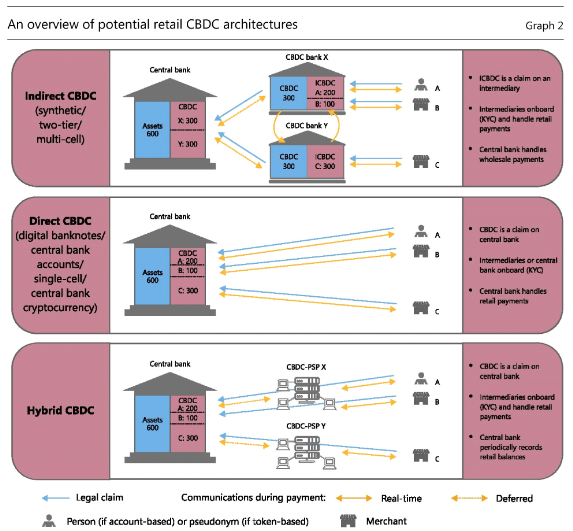
\includegraphics[width=1.0\linewidth]{Figure/chp2/image3.png} % Adjust path as needed
    \caption{An overview of potential retail CBDC architectures: Indirect, Direct, and Hybrid models. \\
    (Source: Bank for International Settlements (BIS), \textit{Authors’ elaboration}, 2022.)}
    \label{fig:1}
\end{figure}

\noindent
This figure illustrates three main CBDC architectures. In all models, the central bank issues the CBDC. The \textbf{Indirect CBDC} model uses intermediaries who onboard consumers and handle retail payments, while the central bank manages wholesale payments. The \textbf{Direct CBDC} model places the central bank in direct control of all retail payments and customer accounts. The \textbf{Hybrid CBDC} model combines features of both, with intermediaries managing retail payments but the central bank maintaining a copy of retail holdings for resilience. Each model supports either account-based or token-based access.

\section{Global CBDC Initiatives}
Several countries have either launched or piloted CBDC programs, some of them are mentioned below:

\begin{itemize}
    \item \textbf{e-CNY (China):} One of the most advanced retail CBDC pilots, designed for everyday transactions with tiered privacy.
    \item \textbf{Sand Dollar (Bahamas):} A fully deployed CBDC aimed at improving financial inclusion across the islands.
    \item \textbf{Digital Euro (EU):} A work-in-progress initiative focusing on maintaining monetary sovereignty in the eurozone.
    \item \textbf{Project Dunbar (BIS):} A multi-CBDC platform for cross-border transactions involving several central banks.

\begin{figure}[H]
    \centering
    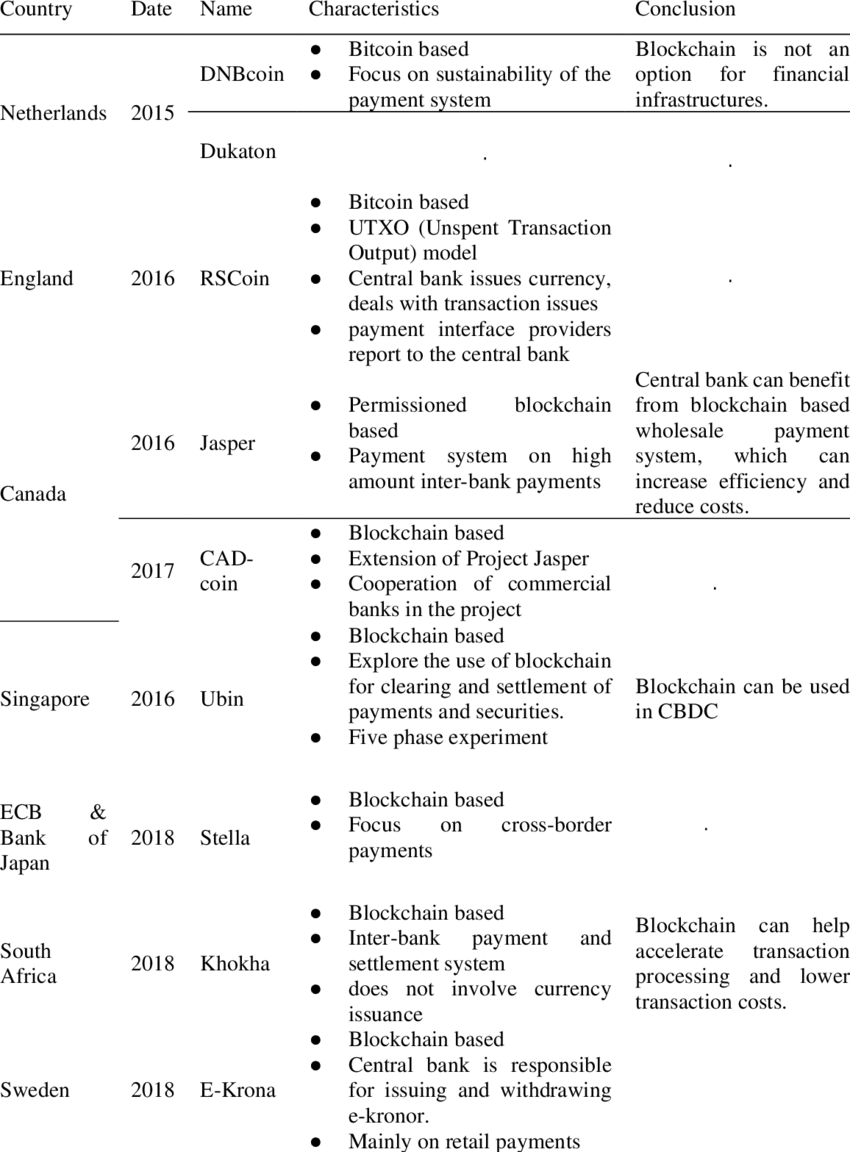
\includegraphics[width=0.9\linewidth]{Figure/chp2/image.png}
 \caption{CBDC projects in different countries.\\
 (Reproduced from Tayazime \& Moutahaddib (2023), \textit{European Scientific Journal}, 19(16), 160. DOI: \url{https://doi.org/10.19044/esj.2023.v19n16p160}. Licensed under CC BY-NC-ND 4.0.)}
  --
    \label{fig:fig2}
\end{figure}

\vspace{3cm}

\section{India’s Digital Payment Ecosystem}
India has a robust and rapidly evolving digital payment system which includes:

\begin{itemize}
    \item \textbf{UPI (Unified Payments Interface):} A real-time payment system facilitating inter-bank transactions via mobile devices.
    \begin{itemize}
        \item \textbf{NEFT/RTGS:} Traditional centralized systems for high-value and batch-based payments.
    \end{itemize}
    \item \textbf{e-Wallets:} Widely used platforms like Paytm and PhonePe for small retail transactions.
\end{itemize}

The Reserve Bank of India (RBI) has also launched pilot projects for both \textbf{wholesale} and \textbf{retail} CBDCs, indicating its interest in exploring state-backed digital currencies.

\section{Limitations in Existing Literature}
Although several international models of CBDCs exist, most are not directly transferable to the Indian context due to differences in infrastructure, financial inclusion levels, and regulatory structures. Key gaps include:

\begin{itemize}
    \item Lack of focus on \textbf{offline transactions} in rural or low-connectivity regions.
    \item Inadequate treatment of \textbf{privacy and data localization} concerns.
    \item Absence of a model that integrates seamlessly with \textbf{existing systems} like UPI.
\end{itemize}

\section{Summary}
This chapter has been precise to show the different perspective and ideas related to digital currencies that are being globally applied, reviewed current CBDC models, and identified critical gaps. A good understanding of present payment methods in India. These insights will further provide the foundation for the proposed CBDC model in the next coming chapter.
